
\let\negmedspace\undefined
\let\negthickspace\undefined
\documentclass[journal]{IEEEtran}
\usepackage[a5paper, margin=10mm, onecolumn]{geometry}
%\usepackage{lmodern} % Ensure lmodern is loaded for pdflatex
\usepackage{tfrupee} % Include tfrupee package

\setlength{\headheight}{1cm} % Set the height of the header box
\setlength{\headsep}{0mm}     % Set the distance between the header box and the top of the text

\usepackage{gvv-book}
\usepackage{gvv}
\usepackage{cite}
\usepackage{amsmath,amssymb,amsfonts,amsthm}
\usepackage{amsmath}
\usepackage{algorithmic}
\usepackage{graphicx}
\usepackage{textcomp}
\usepackage{xcolor}
\usepackage{txfonts}
\usepackage{listings}
\usepackage{enumitem}
\usepackage{mathtools}
\usepackage{gensymb}
\usepackage{comment}
\usepackage[breaklinks=true]{hyperref}
\usepackage{tkz-euclide} 
\usepackage{listings}
% \usepackage{gvv}                                        
\def\inputGnumericTable{}                                 
\usepackage[latin1]{inputenc}                                
\usepackage{color}                                            
\usepackage{array}                                            
\usepackage{longtable}                                       
\usepackage{calc}                                             
\usepackage{multirow}                                         
\usepackage{hhline}                                           
\usepackage{ifthen}                                           
\usepackage{lscape}
\usepackage{circuitikz}
\tikzstyle{block} = [rectangle, draw, fill=blue!20, 
    text width=4em, text centered, rounded corners, minimum height=3em]
\tikzstyle{sum} = [draw, fill=blue!10, circle, minimum size=1cm, node distance=1.5cm]
\tikzstyle{input} = [coordinate]
\tikzstyle{output} = [coordinate]


\begin{document}

\bibliographystyle{IEEEtran}
\vspace{3cm}

\title{4.12.23}
\author{AI25BTECH11018-Hemanth Reddy}
 \maketitle
% \newpage
% \bigskip
{\let\newpage\relax\maketitle}

\renewcommand{\thefigure}{\theenumi}
\renewcommand{\thetable}{\theenumi}
\setlength{\intextsep}{10pt} % Space between text and floats


\numberwithin{equation}{enumi}
\numberwithin{figure}{enumi}
\renewcommand{\thetable}{\theenumi}

\textbf{Question:}\\


A point moves so that square of its distance from the point (3, -2) is numerically
equal to its distance from the line 5x - 12y = 3. The equation of its locus is


\textbf{Solution:}\\

\begin{align}
   \text{ Let the position vector of point }  \vec{P} \text{ is }
   = \myvec{ x \\ y} \\
  \text{  Let }\vec{a} = \myvec{ 3 \\ -2} 
\end{align}
Square of distance of point $\vec{P}$ from $\vec{a}$ is $\norm{\vec{P} -\vec{a} }^{2}$ = $(\vec{P} -\vec{a})^{T} (\vec{P} -\vec{a})$\\

\begin{align}
    (\vec{P} -\vec{a}) = \myvec{ x-3 \\ y+2} 
\end{align}

\begin{align}
    (\vec{P} -\vec{a})^{T}(\vec{P} -\vec{a})= \myvec{ x-3 & y+2}\myvec{ x-3 \\ y+2} = (x-3)^{2}+(y+2)^{2}
\end{align}
\begin{align}
     \text{Let} \quad \vec{n} = \myvec{ 5 \\-12}  \\
     |\textbf{n}| = \sqrt{\textbf{n}^T \textbf{n}} = \sqrt{\myvec{ 5 & -12} \myvec{ 5 \\-12}} = \sqrt{25+144} = 13 
\end{align}

\begin{align}
    d = \frac{|\textbf{P}^T \textbf{n} - 3|}{|\textbf{n}|} = \frac{|5x - 12y - 3|}{13}
\end{align}

\begin{align}
   (x-3)^{2}+(y+2)^{2}= d = \frac{|5x - 12y - 3|}{13}
\end{align}

 
\begin{align}
 (x-3)^{2}+(y+2)^{2}= \frac{(5x - 12y - 3)}{13}\\
13x^2 + 13y^2 - 83x + 64y + 172 = 0
\end{align}



The locus of the point is a circle.

\begin{figure}
    \centering
    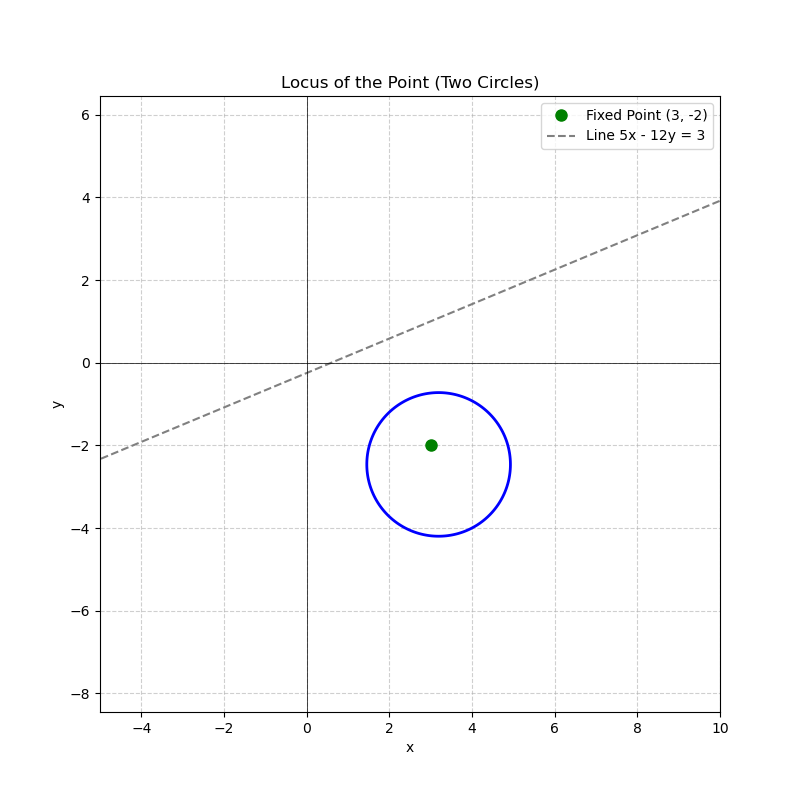
\includegraphics[width=0.8\linewidth]{figs/circle.png}
    \caption{}
    \label{fig:placeholder}
\end{figure}
\end{document}
